\chapter{Efeito Castanha do Pará - \textit{Brazil Nut Effect (BNE)}}
\label{chap:BNE}
    Historicamente, o fenômeno conhecido como efeito castanha do Pará deu-se em função das exportações da castanha do Pará em contêineres, por navios, e sempre que chegavam ao destino, observam-se que as maiores castanhas estavam no topo. Inicialmente pensou-se que os comerciantes brasileiros arranjavam as castanhas de modo que as maiores estivessem em cima e, as menores e quebradas em baixo. Após investigação, foi verificado que as castanhas maiores ascendiam devido a vibração que os contêineres sofriam ao longo do transporte, por isso o efeito ficou conhecido como efeito castanha do Pará, ou \textit{Brazil Nut Effect (BNE)} \cite{Caio-Tese}.

    O BNE ocorre quando um grão, maior que os grãos do meio, sobe contra a gravidade no meio granular agitado. Este fenômeno está associado com a fase granular do sistema. Num sistema granular sólido, o grão maior fica estático. Com o aumento da agitação, o sistema passa para o estado líquido, permitindo que haja movimentação dos grãos no sistema \cite{Why_the_Brazil_nuts_are_on_top}. A movimentação do material ocorre em correntes de convecção que se formam próximas das paredes e pelo preenchimento do espaço anteriormente ocupado pelo grão maior, com o efeito catraca \cite{Inertia_in_the_Brazil_nut_problem, The_water-enhance_Brazil_nut_effect}.

    Vários diagramas de fase foram observados para alguns dos parâmetros do BNE. Dentre as principais variáveis estão a razão de diâmetros dos grãos e a razão de densidades \cite{A_Horizontal_Brazil-Nut_Effect_and_Its_Reverse, Brazil-Nut_effect_Size_separation_of_granular_particles, Brazil-nut_effect_versus_reverse_Brazil-nut_effect_in_a_moderately_dense_granular_fluid, Categorization_of_Brazil_nut_and_its_reverse_under_less-convective_conditions_for_microgravity_geology, Competition_of_Brazil_nut_effect_buoyancy_and_inelasticity_induced_segregation_in_a_granular_mixture, Reverse_Brazil_Nut_Problem_Competition_between_Percolation_and_Condensation, Reversing_the_Brazil-Nut_Effect_Competition_between_Percolation_and_Condensation, Reverse_buoyancy_in_a_vibrated_granular_bed_Computer_Simulations, Scaling_behavior_in_convection-driven_Brazil-nut_effect, Segregation_in_a_fluidized_binary_granular_mixture_Competition_between_buoyancy_and_geometric_forces, Simple_model_for_reverse_buoyancy_in_a_vibrated_granular_system}. Dentro das caracterizações dos planos de fase, a aceleração adimensional, mostrado na equação \ref{equ:gamma}, é o parâmetro de comparação relacionado à subida do intruso.
\begin{equation}
    \label{equ:gamma}
    \Gamma = \frac{A\omega^{2}}{g},
\end{equation}
em que $\Gamma$ é o adimensional, $A$ é a amplitude de vibração do sistema, $\omega$ é a frequência de vibração e $g$ é o valor da gravidade.

    Nesta parte da tese, utilizaremos $2500$ grãos. O diâmetro médio do grão é $d = 1\pm 2.5\%$, distribuídos uniformemente. O diâmetro do intruso é de $D = 5$ vezes o diâmetro médio dos grãos. A densidade de todos os grãos é a mesma, e vale $\rho = 1/\pi$, e portanto a massa média dos grãos é de $m = 0,25$, exceto quando estiver ressaltado nas figuras. A constante de mola na direção normal é de $k_{n} = 1000$ e a tangencial é de $k_{t} = 750$. A atuação do amortecedor é no regime crítico ($\gamma = 2\sqrt{m k}$), e vale aproximadamente $\gamma = \sqrt{10}$. O atrito dos grãos valem $\mu = 0,5$, tanto entre grãos, quanto entre paredes, quando houver. O passo de tempo ($dt=pT$) vale aproximadamente $dt = \frac{1}{2000\sqrt{10}}$, utilizando a fração de $p=0,01$ do período de oscilação do modelo de contato massa mola $T = \sqrt{\frac{m}{k}}$. A largura da caixa é de $L = 37.5$ diâmetros de grão.

    Inicialmente, estudamos o sistema com paredes no fundo e nas laterais, formando uma caixa. Observamos nestas simulações correntes de convecção próximos às paredes.

\begin{figure}
    \centering
    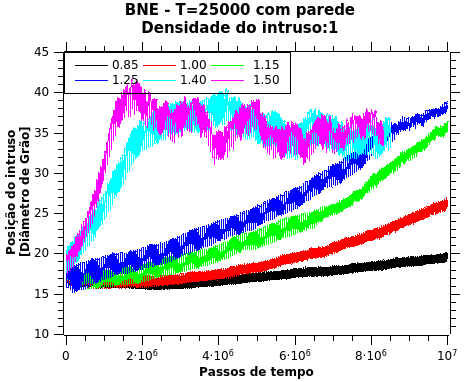
\includegraphics[width=0.45\textwidth]{04-figuras/BNE25000D1.png}
    \caption{Média de $10$ amostras da subida do intruso em função do adimensional de aceleração. O período de agitação é de $25000$ passos de tempo em uma forma senoidal. Este sistema possui atrito nas paredes e densidade do intruso igual a dos grãos.}
    \label{fig:BNE25000_Parede}
\end{figure}

\begin{figure}
    \centering
    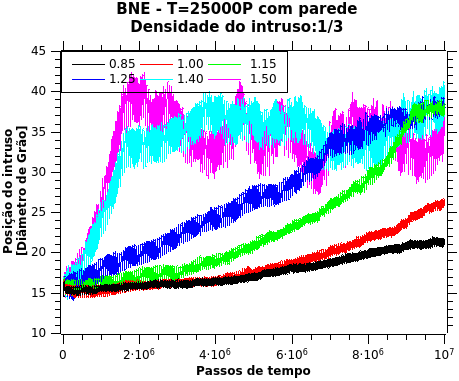
\includegraphics[width=0.45\textwidth]{04-figuras/BNE25000D1-3.png}
    \caption{Média de $5$ amostras da subida do intruso em função do adimensional de aceleração. O período de agitação é de $25000$ passos de tempo em uma forma senoidal. Este sistema possui atrito nas paredes e densidade do intruso é $\frac{1}{3}$ da densidade dos grãos.}
    \label{fig:BNE25000_Parede_Densidade1-3}
\end{figure}

\begin{figure}
    \centering
    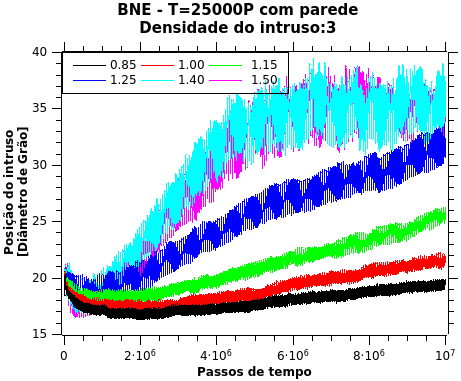
\includegraphics[width=0.45\textwidth]{04-figuras/BNE25000D3.png}
    \caption{Média de $5$ amostras da subida do intruso em função do adimensional de aceleração. O período de agitação é de $25000$ passos de tempo em uma forma senoidal. Este sistema possui atrito nas paredes e densidade do intruso é $3$ vezes a densidade dos grãos.}
    \label{fig:BNE25000_Parede_Densidade3}
\end{figure}

    Percebemos que intrusos mais densos sobem mais lentamente que intrusos menos densos. Os tempos de subida, quando comparados, podem ser ordenados das figuras $\ref{fig:BNE25000_Parede_Densidade1-3} < \ref{fig:BNE25000_Parede} < \ref{fig:BNE25000_Parede_Densidade3}$. Assim como as correntes de convecção são mais intensas, o intruso sobe mais rapidamente e cai mais rapidamente, visto na amplitude de $\Gamma = 1,5$ para as figuras \ref{fig:BNE25000_Parede_Densidade1-3}, \ref{fig:BNE25000_Parede} e \ref{fig:BNE25000_Parede_Densidade3}, respectivamente.

    Quando retirado o atrito entre os grãos e as paredes, temos que o efeito da convecção no sistema diminui, ocasionando em uma subida mais lenta que quando o atrito está presente. A figura \ref{fig:BNE25000_sem_Atrito_Parede} mostra a subida do intruso no sistema em que as paredes não possuem atrito.

\begin{figure}
    \centering
    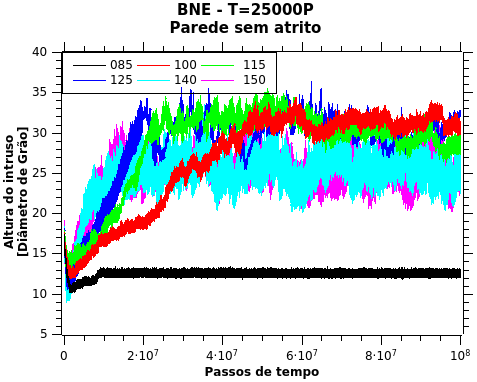
\includegraphics[width=0.45\textwidth]{04-figuras/BNE25000PsemAtrito.png}
    \caption{Média de $3$ amostras da subida do intruso em função do adimensional de aceleração. O período de agitação é de $25000$ passos de tempo em uma forma senoidal. Este sistema não possui atrito nas paredes.}
    \label{fig:BNE25000_sem_Atrito_Parede}
\end{figure}

    Ao comparar os tempos de subida do sistema que possui atrito nas paredes (figura \ref{fig:BNE25000_Parede}) com o sistema que não possui atrito nas paredes (figura \ref{fig:BNE25000_sem_Atrito_Parede}), percebemos que o tempo de subida é maior, além de que o sistema que possui agitação menor que a gravidade não sobe, mostrando que um dos fatores que importam para o \textit{BNE} são as correntes de convecção formadas próximas das paredes.

    Quando retiramos o atrito do sistema, o intruso chega ao fundo do sistema, independente da amplitude de vibração. A figura \ref{fig:BNE25000_sem_Atrito} exibe o comportamento do intruso para o sistema sem atrito.

\begin{figure}
    \centering
    \begin{minipage}{.45\linewidth}
        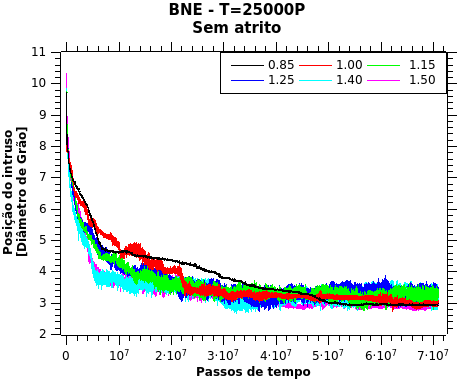
\includegraphics[width=0.9\textwidth]{04-figuras/BNE25000semAtrito.png}
        \subcaption{Diferentes amplitudes}
        \label{fig:BNE25000_sem_Atrito_Sistema}
    \end{minipage}
    \begin{minipage}{.45\linewidth}
        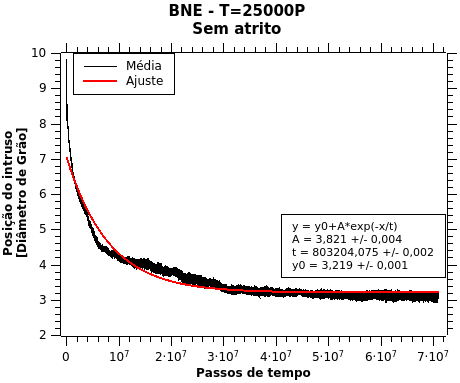
\includegraphics[width=0.9\textwidth]{04-figuras/BNE25000semAtrito_Ajuste.png}
        \subcaption{Ajuste da média}
        \label{fig:BNE25000_sem_Atrito_Ajuste}
    \end{minipage}
    \caption{Amostra da queda do intruso em função do adimensional de aceleração. O período de agitação é de $25000$ passos de tempo em uma forma senoidal. Este sistema não possui atrito. A figura \ref{fig:BNE25000_sem_Atrito_Ajuste} possui a média das curvas apresentadas na figura \ref{fig:BNE25000_sem_Atrito_Sistema} e uma o ajuste de um decaimento exponencial em função do tempo, da posição do intruso até o fundo do sistema.}
    \label{fig:BNE25000_sem_Atrito}
\end{figure}

    Se ao invés de retirarmos o atrito, retirarmos as paredes laterais formando uma condição periódica de contorno de largura $28$ diâmetros de grão, verificaremos que o \textit{BNE} não acontece para o período de vibração de $25000$ passos de tempo, como mostrado na figura \ref{fig:BNE25000_Contorno}.

\begin{figure}
    \centering
    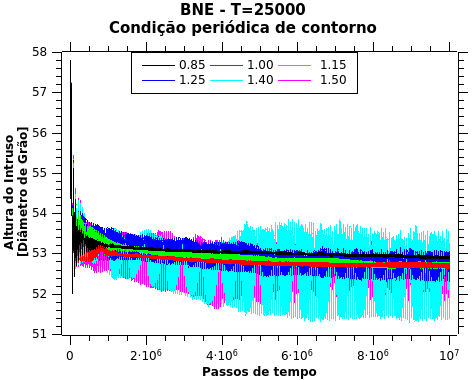
\includegraphics[width=0.45\textwidth]{04-figuras/BNE25000Contorno.png}
    \caption{Média de $5$ amostras da posição do intruso em função do adimensional de aceleração. O período de agitação é de $25000$ passos de tempo em uma forma senoidal. Este sistema não possui paredes, mas condição periódica de contorno.}
    \label{fig:BNE25000_Contorno}
\end{figure}

    Já no caso de períodos maiores, o BNE ocorre. A figura \ref{fig:BNE30000_Contorno} exemplifica o \textit{BNE} ocorrendo com condição periódica de contorno e período de vibração de $30000$ passos de tempo.

\begin{figure}
    \centering
    \begin{minipage}{.45\linewidth}
        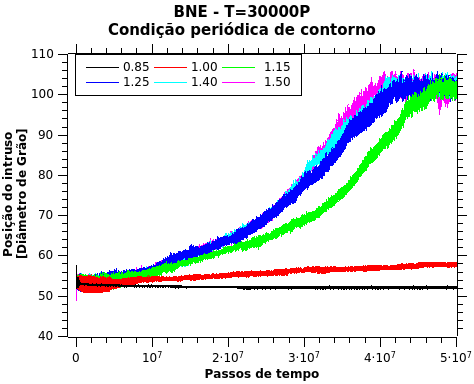
\includegraphics[width=0.9\textwidth]{04-figuras/BNE30000Contorno.png}
        \subcaption{Média das amostras}
        \label{fig:BNE30000_Contorno_Media}
    \end{minipage}
    \begin{minipage}{.45\linewidth}
        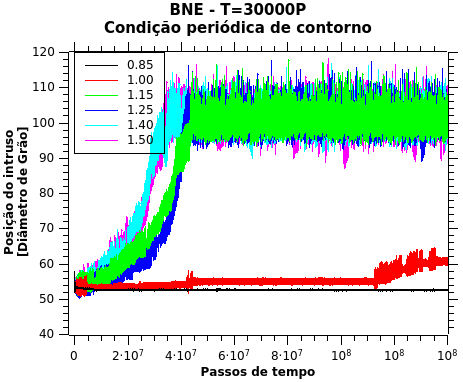
\includegraphics[width=0.9\textwidth]{04-figuras/BNE30000Contorno1.png}
        \subcaption{Amostra mais longa}
        \label{fig:BNE30000_Contorno1}
    \end{minipage}
    \caption{Média de $10$ amostras da subida do intruso em função do adimensional de aceleração. O período de agitação é de $30000$ passos de tempo em uma forma senoidal. Este sistema não possui paredes, mas condição periódica de contorno. A figura \ref{fig:BNE30000_Contorno1} mostra a amostra com maior passos de tempo de simulação.}
    \label{fig:BNE30000_Contorno}
\end{figure}

    Na figura \ref{fig:BNE30000_Contorno1}, percebemos que acelerações menores que a gravidade não fazem o intruso ascender, enquanto acelerações próximas da gravidade tem um movimento de ascensão lento e em saltos. Por não haver paredes, as correntes de convecção não se formam no sistema, o que faz com que o intruso atinja o topo e não desça mais.

%    Com estes resultados, submetemos um artigo para a publicação ... \textbf{Parte necessária para a qualificação}.

    No próximo capítulo, descreveremos os modos de transporte de grãos quando arrastados por um fluido.

%    Inertia_in_the_Brazil_nut_problem -> Atribui a convecção ao atrito das paredes e colapsa as curvas de ascensão.
%    The_water-enhance_Brazil_nut_effect -> Uso do fluido intersticial com BNE.
%    Why_the_Brazil_Nuts_are_on_top -> Atribui o BNE ao efeito catraca, usando Monte Carlo e desprezando atrito e a massa é desprezível para o efeito.
%    A_Horizontal_Brazil-Nut_Effect_and_Its_Reverse -> Vibra horizontalmente e com diferentes materiais (densidades), reproduz BNE (ida para o centro) e rBNE (ida para as bordas). Frequências de 0.5 à 2Hz, amplitude de $3,175n$mm, com $n$ variando de $3 ... 7$, diâmetro médio dos grãos de 6mm, diâmetro do intruso $1,3 ... 7$ vezes o diâmetro dos grãos e coeficiente de atrito de $0,67$. Exibe um diagrama de fase Diâmetro/Densidade.
%    Brazil-Nut_effect_Size_separation_of_granular_particles -> Descreve o fenômeno em função do diâmetro e da densidade, fixa a frequência em $13$Hz e a amplitude em $7,35$mm e o diâmetro do grão menor em $0,5$mm, ou seja, a relação amplitude e diâmetro do grão é de $14,7$ vezes. Diâmetro do intruso pode chegar à $25,4$mm, o equivalente $50800$ vezes o diâmetro do grão.
%    Brazil-nut_effect_versus_reverse_Brazil-nut_effect_in_a_moderately_dense_granular_fluid -> Analítico/teórico sobre os planos de fase das regiões BNE e rBNE em função do diagrama Diâmetro/Densidade com coeficiente de compactação e restituição.
%    Caracterization_of_Brazil_nut_and_its_reverse_under_less-convective_conditions_for_microgravity_geology -> Reproduz o BNE em condição fechada, porém com atrito baixo entre parede/grão, com condições de aceleração menores q a gravidade.
%    Competition_of_Brazil_nut_effect_buoyancy_and_inelasticity_induced_segregation_in_a_granular_mixture -> Compara os resultados do BNE em função das massas, diâmetros e coeficientes de restituição.
%    Reverse_Brazil_Nut_Problem_Competition_between_Percolation_and_Condensation -> Mostra o diagrama qualitativo da transição BNE para rBNE em função da razão dos diâmetros pelas massas. Relaciona a temperatura granular.
%    Reverse_buoyancy_in_a_vibrated_granular_bed_Computer_Simulations -> Insere um fluido como amortizador e demonstra as forças e seus efeitos.
%    Reversing_the_Brazil-Nut_Effect_Competition_between_Percolation_and_Condensation -> Mostra o diagrama BNE/rBNE em função da densidade versus diâmetro, com o diagrama de frequência por aceleração normalizada.
%    Scaling_behavior_in_convection-driven_Brazil-nut_effect ->  mostra o esquema de convecção para a contribuição no BNE
%    Segregation_in_a_fluidized_binary_granular_mixture_Competition_between_buoyancy_and_geometric_forces -> Diagrama BNE/rBNE densidade versus diâmetro
%    Simple_model_for_reverse_buoyancy_in_a_vibrated_granular_system -> Velocidade no BNE/rBNE densidade
%    Study_the_effect_of_vibration_frequency_and_amplitude_on_the_quality_of_fluidization_of_a_vibrated_granular_flow_using_discrete_element_method -> Caracteriza o fluido em função da altura do sistema.

%    Size_separation_in_vibrated_granular_matter -> Compilado dos artigos acima

%    Convection_Cells_in_Vibrating_Granular_Media -> Em relação ao BNE não é mostrado, uma vez q a distribuição dos raios dos grãos são próximas entre si. Mostra a convecção na agitação dos granulares, mesmo quando possuem condição periódica de contorno. Porém a agitação é muito alta.
